%\chapter{Monitoring}
%\label{ch:monitoring}

%One of the disadvantages of a microservice architecture is the amount of information it produces and requires the user to keep up with.
With the growth of the microservices industry, and as a new way of constructing applications, microservices' availability, performance, and functionality becomes a concern that everyone cares about. Stakeholders want to make sure each end-user has a good experience, operations teams want to ensure applications are available and performing well, and development teams want the applications and microservices to function as designed.

Even though everything most services are decoupled, some still rely on communication between them and as such, if a component deteriorates or fails, it can still affect the applications performance or eventually lead to application failure. Understanding how each component is performed is essential to gauge the real health and status of the application as a whole. This monitoring can help the team:

\begin{itemize}
    \item Understand the overall health of the application
    \item Gain insight into the performance of each individual service
    \item Ensure that transactions are available and performing well
    \item Understand the load of each service (i.e., maybe a feature is not being used and can be replaced by something else or removed entirely)
    \item Optimize end-user experience
\end{itemize}

However, gathering all these metrics and reading them from massive text files still does not solve the problem at hand. As such, visualization tools were introduced, which allow for an easier real-time overview of data. This tools consume the logs produced by the monitoring tools and allow the exploration of such data with filtering and grouping. For example, instead of having the current number of users constantly updated without having a way to see previous values, we can now trace a graph of concurrent users which allows us to understand how it is progressing.

The following section \ref{ss:monitoring-implementations} will detail some of the tools currently available for monitoring and visualization, followed by an description of how they were integrated into our system in Section \ref{ss:monitoring-solution}.

%\subsection{Problem}
%\label{s:6_problem}

\subsection{Implementations}
\label{ss:monitoring-implementations}

The following sections describe the tools found that could aid us with the monitoring process and everything the precedes it such metric scraping and the tools to helps us visualize all of this information.

\subsubsection{Prometheus}
\label{sss:prometheus}
%% -- Created: 03-07-21
%% -- Last edit: 05-07-21

Prometheus \footnote{\url{https://www.prometheus.io/}} is an open-source monitoring system which collects metrics, evaluates expressions, offers visualization dashboards and has alert mechanisms. Its main features are~\cite{prometheus-overview}:

\begin{itemize}
    \item A multidimensional data model with time series data identified by metric name and key/value pairs (e.g. <metric name>\{<label name>=<label value>, ...\});
    \item \textbf{PromQL} a flexible query language to leverage this dimensionality;
    \item Autonomous single server nodes, as such, no reliance on distributed storage;
    \item Time series collections occurs via a \gls{pull-model} over \acrshort{http};
    \item Monitored nodes (targets) are discovered via service discovery or static configuration
\end{itemize}

\paragraph{Architecture}
%\label{sss:prometheus-architecture}

The prometheus ecosystem consists of multiple components, some of which can see be seen in Fig. \ref{fig:prometheus-architecture}.

\begin{figure}[h]
    \centering
    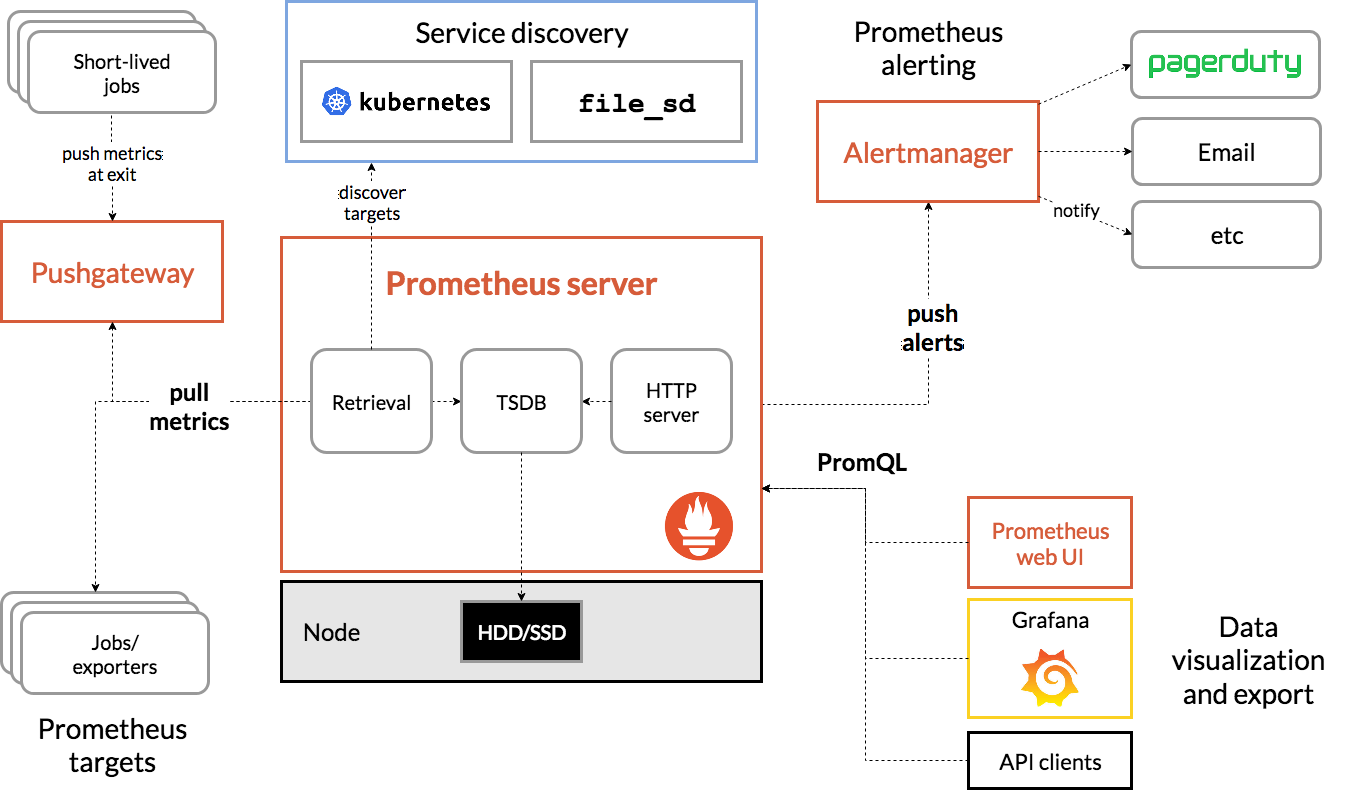
\includegraphics[width=1\textwidth,clip,trim=0 0 0 0]{Chapters/img/2_background/prometheus-architecture.png}
    \caption{Prometheus architecture~\cite{prometheus-overview}} 
    \label{fig:prometheus-architecture}
\end{figure}

The main components are:

\begin{itemize}
    \item \textbf{Prometheus server:} scrapes metrics from one or more targets and stores them in a \acrlong{tsdb} (\acrshort{tsdb});
    \item \textbf{Client-libraries:} there are multiple available libraries to match the language used in the application, that let the user define and expose internal metrics via an \acrshort{http} endpoint on the application instance;
    \item \textbf{Push gateway:} Support short-lived jobs, who push communication to announce their metrics. Since these kind of jobs may not exist long enough to be scrap, they are pushed to the push gateway, who then exposes these metrics to prometheus; 
    \item \textbf{Exporters:} monitor third-party systems to convert the existing metrics into the prometheus data model;
    \item \textbf{Alertmanager:} Handles alerts sent by client applications such as the Prometheus server. It takes care of deduplicating, grouping and routing them to the correct third-party notification platforms such as email.
    
\end{itemize}

Prometheus was chosen due to its popularity in the industry and for being an open-source project. It can easily be customized to our needs if required, and most of all its easy to scrape metrics from other software allowing for easier integration with the current system.


%------------------------------------------%------------ Grafana -----------------------------
\subsubsection{Grafana}
\label{sss:grafana}
%% -- Created: 03-07-21
%% -- Last edit: 05-07-21

Grafana~\footnote{\url{https://grafana.com/}} is a cross platform open-source measurement, analysis and visualization tool, which can query the collected data and present it through multiple dashboards. 

Grafana monitoring is achieved using panels, which is the basic building block for visualization in Grafana, and those panels can contain graphs, tables, text, or custom plugins (i.e. a clock or map). As such, a dashboard is a collection of panels, each of which holds a set of variables (server, application, sensor name) arranged in a grid, which the user can change the observed data by switching variables. An example of a dashboard can be seen in Fig. \ref{fig:grafana-example}.

\begin{figure}[h]
    \centering
    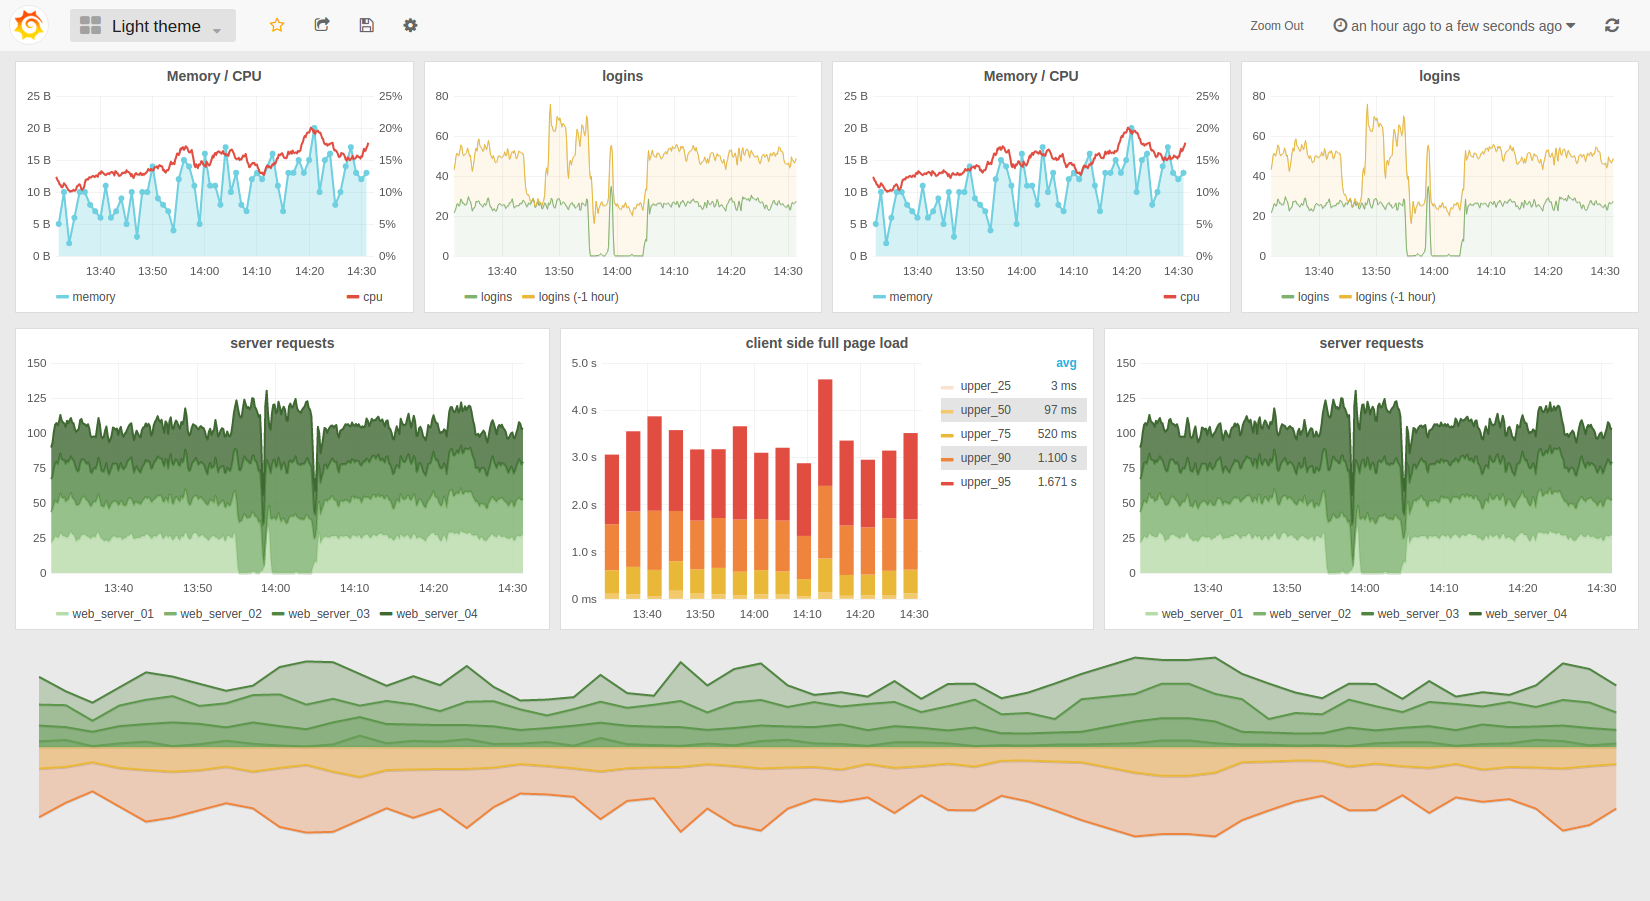
\includegraphics[width=1\textwidth,clip,trim=0 0 0 0]{Chapters/img/2_background/grafana-example.png}
    \caption{Grafana dashboard~\cite{grafana-example}} 
    \label{fig:grafana-example}
\end{figure}

Its main features are~\cite{grafana-features}:

\begin{itemize}
    \item \textbf{Dashboard templating}: It allows the users to create a dashboard to suit their needs, without almost no restrictions, they are extremely adaptable. Templating lets data be examined at every level from macro to micro (e.g., starting with a whole country and drilling down to a particular region). The dashboards are then shareable with everyone;
    \item \textbf{Provisioning:} It provides provisioning so the setup can be automated using a script. For instance, to create a new Kubernetes cluster, it is possible to have Grafana automatically help with a script that already has the right server, IP address, and data sources set up and locked;
    \item \textbf{Annotations:} It is possible to manually annotate data, which is particularly helpful to correlate data when something goes wrong; 
    \item \textbf{Kiosk mode}: dashboards can be selected to create a playlist, this playlist can now be displayed in a TV or monitor to cycle throughout the day;
    \item \textbf{Teams and permissions:} Dashboards can be limited to specific teams, allowing only determined dashboards to be viewed by teams in charge of that service.
\end{itemize}

One of the most common alternatives to Grafana is \textbf{Kibana}~\footnote{\url{https://www.elastic.co/kibana/}}, where the key difference between the two tools stems from their purpose. Grafana design caters to analyzing and visualizing metrics such as memory, CPU, disk, and I/O utilization. It does not allow full-text data querying. Kibana, on the other hand, runs on top of Elasticsearch and is used primarily to visualize and analyse log messages. They are both useful in their respective fields, but for this thesis Grafana served our needs better.


\subsection{Solution}
\label{ss:monitoring-solution}

%Even though there were multiple relevant sections to monitor such as databases, code itself through logs, etc... We chose to focus on the well-being and performance of the microservices themselves.
%Começamos por monitorizar os microserviços associados ao backend, criados em Java.

Even through it was possible to monitor and track the entire system, we have decide to focus our efforts on the well-being and performance of backend microservices. Which means we care about what is happening on the pods that are hosting our services. 

Instead of manually exposing each of the resources and setting up each microservice individually, we chose to use the \textit{Spring Boot Actuator}, which adds features to help monitor the service, gather metrics, understand traffic, and even state of the database, all exposed through HTTP endpoints. It includes several endpoints and the possibility of adding custom ones. For the current goal, the following endpoints were considered as the most important:

\begin{itemize}
    \item \textbf{health} shows application health information, such as \textbf{readiness state} which tells whether the application is ready to accept client requests and \textbf{liveness state}, which indicates whether the internal state is valid, if it is broken it means the application itself is in a failed state and cannot recover from it;
    \item \textbf{metrics} shows 'metrics' information for the current application with the support of the Micrometer~\footnote{\url{https://micrometer.io/}} library, an instrumentation library for JVM-based applications designed to add little to no overhead to the metrics collection activity;
    \item \textbf{prometheus} which exposes metrics in an format that can be scraped by a Prometheus server, once again provided by the micrometer library, as it provides a simple facade over the instrumentation clients for the most popular monitor systems, namely Prometheus.
\end{itemize}

Prometheus is then configured to scrape or poll individual app instances for metrics exposed in \textit{/actuator/prometheus}. For this we must create a \textit{scrape configuration}, which specify a set of targets and parameters describing how to scrape them, also known as \textit{jobs}. Listing \ref{lst:prom-params} provides an example of a job created to scrape the actuator metrics from the \textbf{Params} microservice.

\begin{lstlisting}[caption={Prometheus job for params microservice}, label={lst:prom-params}, captionpos=b]
- job_name: 'be-params-actuator-prometheus'
  metrics_path: '/actuator/prometheus'
  scrape_interval: 5s
  static_configs:
  - targets: ['10.111.42.84:8086']
    labels:
      namespace: backend
      pod: be-params-deployment
      service: be-params-services
\end{lstlisting}

%These metrics can then be utilize by Prometheus, which is constantly performing requests to the API and acquiring data. On top of this metric, we can now apply aggregation queries with \textit{PromQL}, which allowed us to retrieve information such as average requests during the last five minutes. 

%\todo[inline]{Mostrar exemplo de uma query e se for preciso mudar o exemplo dado}

However, one of the reasons which led us to implement and expose this metrics is so we could make them readable by \acrshort{k8s}, allowing us to manage the cluster resources in a more efficient manner reacting to the live feed of information, which is made possible with tools such as the \acrshort{hpa}. But, as mentioned previously, the \acrshort{hpa} only works, by default, with metrics provided by \acrshort{k8s} such as CPU and RAM usage. For this reason, we had to use the third party library \textbf{Prometheus Adapter}~\footnote{\url{https://github.com/kubernetes-sigs/prometheus-adapter}}, which when configure allows the \acrshort{k8s} cluster to recognize the metrics made available through Prometheus. 

The adapter determines which metrics to expose, and how to expose them, through a set of "discovery" rules, where each rule is executed independently, and specifies each of the steps the adapter needs to take to expose a metric in the API. The rules can be broken down into four parts:

\begin{itemize}
    \item \textbf{Discovery}, which specifies how the adapter should find all Prometheus metrics for this rule;
    \item \textbf{Association}, which specifies how the adapter should determine which \acrshort{k8s} resources a particular metric is associated with;
    \item \textbf{Naming}, specifies how the adapter should expose the metric in the custom metrics API;
    \item \textbf{Querying}, which specifies how a request for a particular metric on one or more \acrshort{k8s} objects should be turned into a query to Prometheus.
\end{itemize}

An example of such rules can be seen in Listing \ref{lst:prom-adapter-conf}, which highlights the four parts mentioned: discovery is done through the \textit{seriesQuery}, which specifies the Prometheus series query to use to find some set of Prometheus series; association is controlled by the \textit{resource} field, for this specific case with was done through its kubernetes namespace (backend); naming, the process of converting a prometheus metric name into a metric in the custom metrics API, is controlled by the \textit{name} field; and finally, querying through the \textit{metricsQuery} field, which is a Go template that gets turned into a Prometheus query, for this specific an aggregation query was performed with \textit{PromQL}, which used a rate function over a specific metric with information from the previous three minutes, more details will be provided on this later on during the Testing section (\ref{s:testing}).

\begin{lstlisting}[caption={Prometheus adapter configuration}, label={lst:prom-adapter-conf}, captionpos=b]
    - seriesQuery: '{__name__=~"^http_server_requests_seconds_max"}'
    resources:
      overrides:
        namespace:
          resource: namespace
    name:
      matches: "^(.*)_max"
      as: "http_server_requests_seconds_max_rate"
    metricsQuery: 'rate(http_server_requests_seconds_max{uri=~"/v1/params.*"}[3m])'
\end{lstlisting}

All of this became useful while trying to automate the entire system, however personal oversight is also important, and as such, all information was made available for visualization and analysis through Grafana, which unlike \acrshort{k8s}, pairs up easily with Prometheus.

In Grafana, we can now set up dashboards for each microservice with multiple panels displaying information we deem relevant extracted directly from Prometheus. In Fig. \ref{fig:grafana-dashboard} it is possible to observe our main configuration during testing, which allows us to track and understand the performance of our service, from requests received to garbage collector performance. 

A more in-depth explanation of how the setup was used will be given in the \textit{Testing} section (\ref{s:testing}), where it was crucial for setting up the cluster resources. 

\begin{figure}[h]
    \centering
    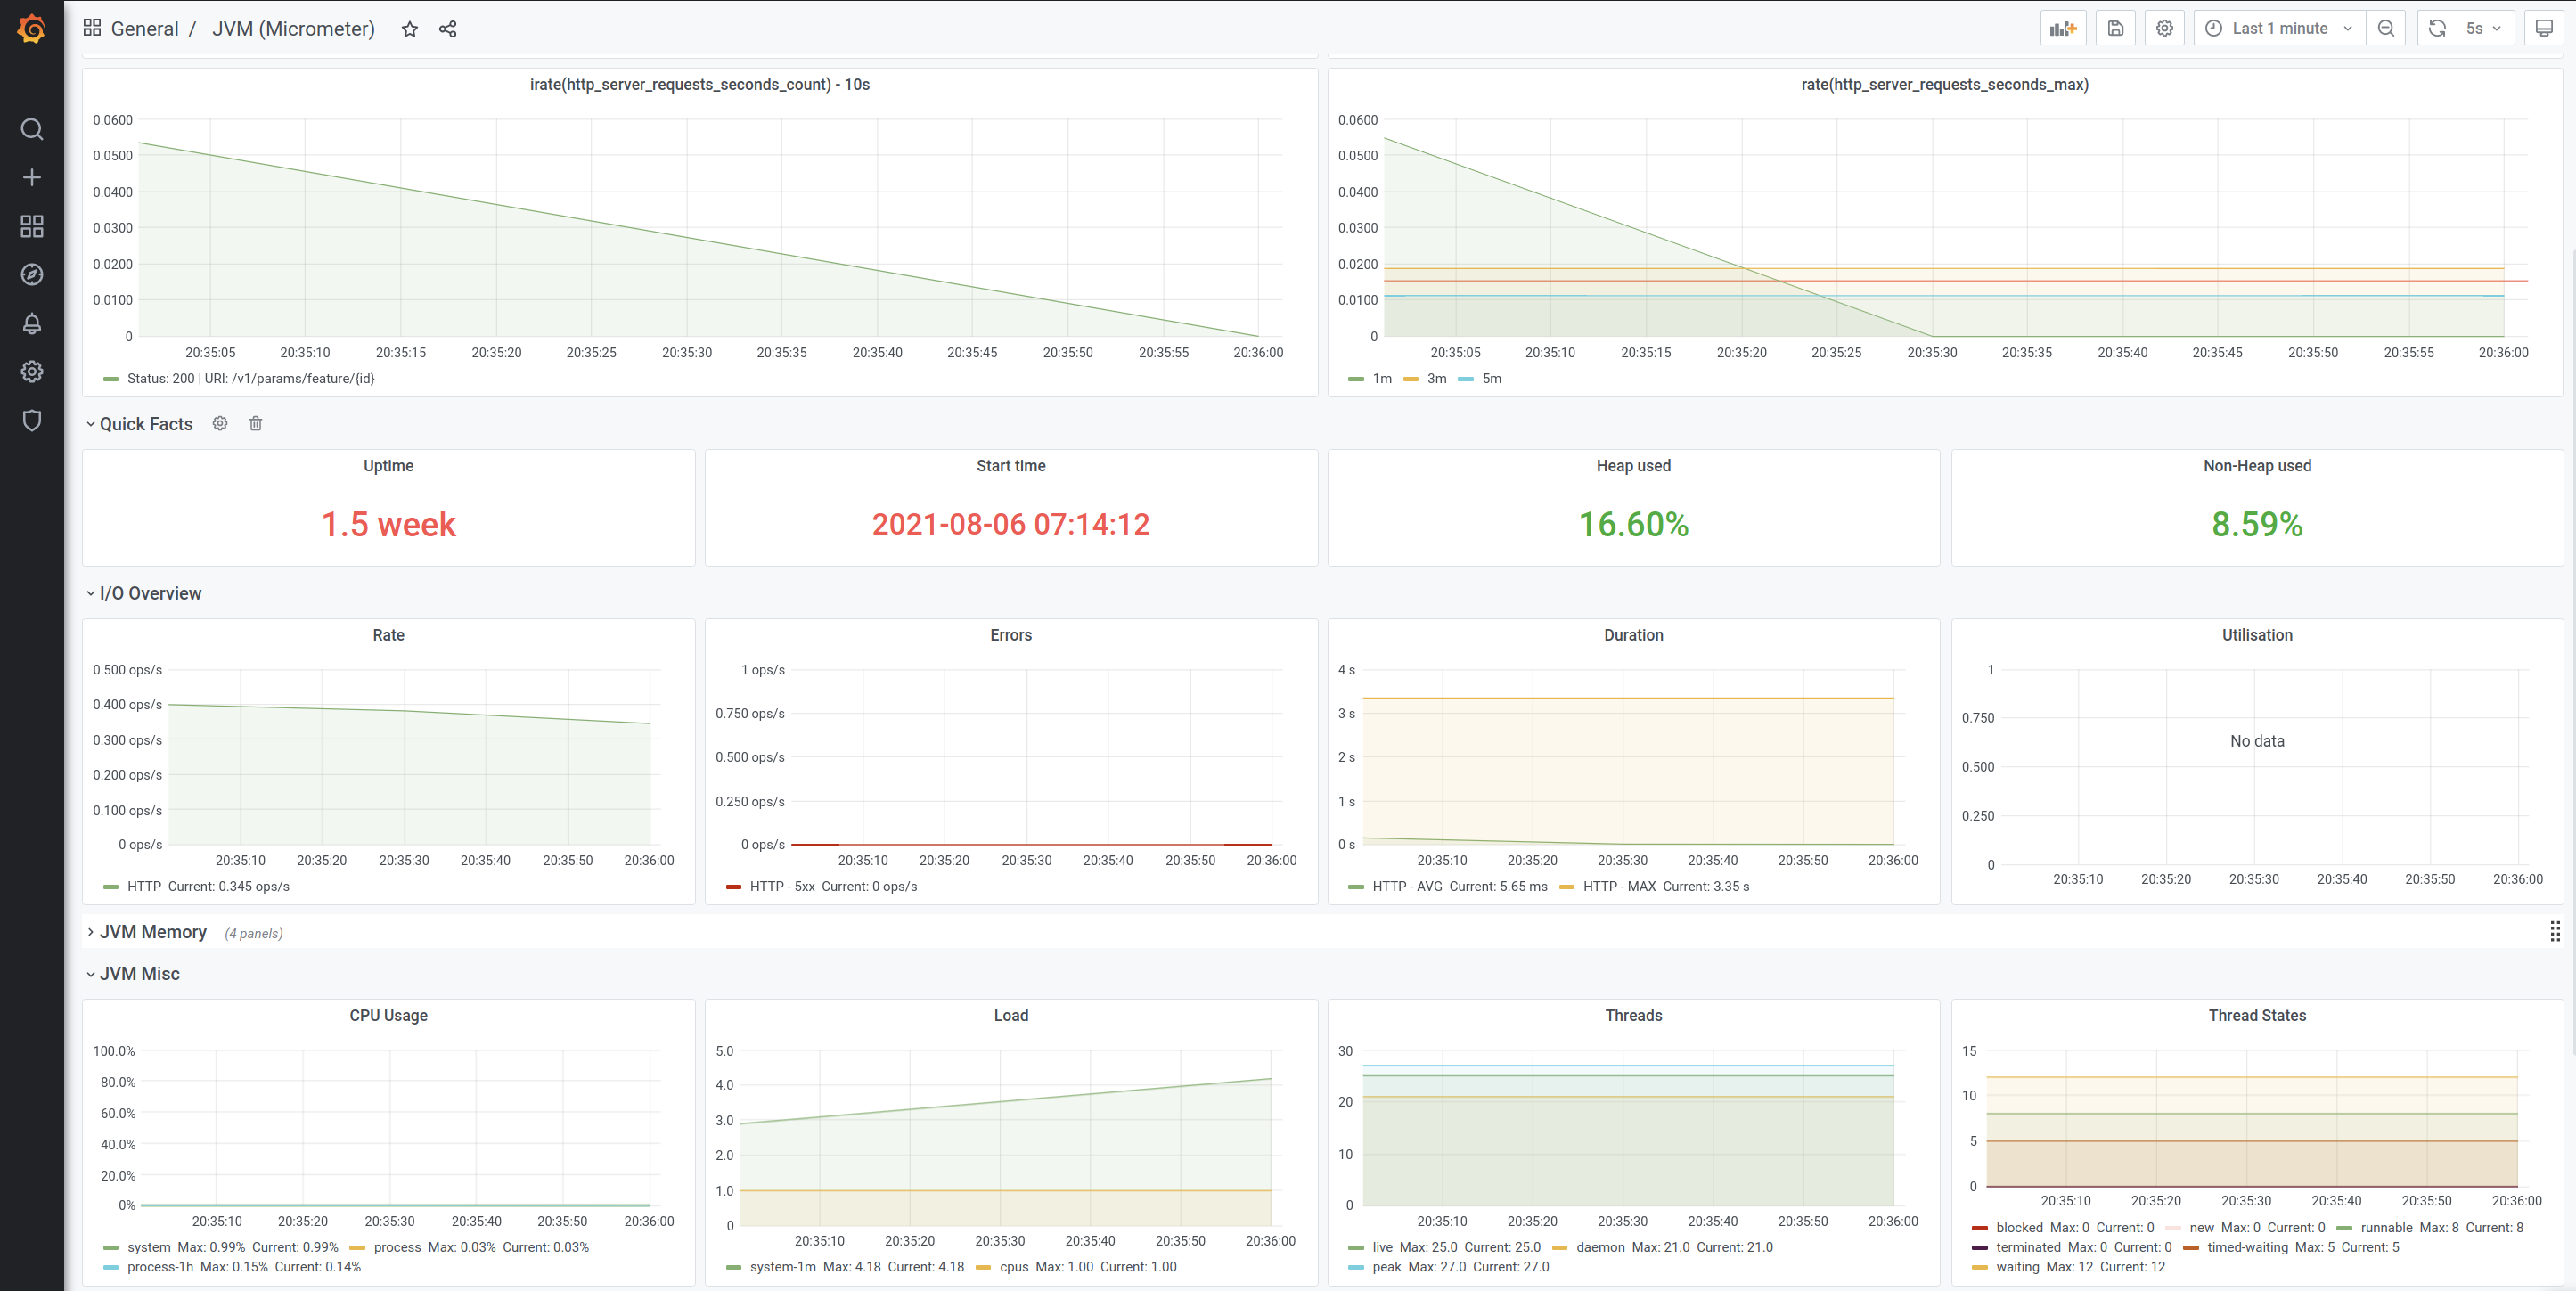
\includegraphics[width=1\textwidth,clip,trim=0 0 0 0]{Chapters/img/backend/grafana-dashboard.png}
    \caption{Grafana dashboard} 
    \label{fig:grafana-dashboard}
\end{figure}

